%% LaTeX Template for ISIT 2018
%%
%% by Stefan M. Moser, October 2017
%%
%% derived from bare_conf.tex, V1.4a, 2014/09/17, by Michael Shell
%% for use with IEEEtran.cls version 1.8b or later
%%
%% Support sites for IEEEtran.cls:
%%
%% http://www.michaelshell.org/tex/ieeetran/
%% http://moser-isi.ethz.ch/manuals.html#eqlatex
%% http://www.ctan.org/tex-archive/macros/latex/contrib/IEEEtran/
%%

\documentclass[conference]{IEEEtran}


%%%%%%
%% Packages:
%% Some useful packages (and compatibility issues with the IEEE format)
%% are pointed out at the very end of this template source file (they are 
%% taken verbatim out of bare_conf.tex by Michael Shell).
%
% *** Do not adjust lengths that control margins, column widths, etc. ***
% *** Do not use packages that alter fonts (such as pslatex).         ***
%
\usepackage[utf8]{inputenc} 
\usepackage[T1]{fontenc}
\usepackage{url}
\usepackage{ifthen}
\usepackage{cite}
\usepackage[cmex10]{amsmath} % Use the [cmex10] option to ensure complicance
                             % with IEEE Xplore (see bare_conf.tex)

\usepackage[color=green!40,textsize=scriptsize]{todonotes}
\usepackage{mathtools}
\mathtoolsset{showonlyrefs}

%% Please note that the amsthm package must not be loaded with
%% IEEEtran.cls because IEEEtran provides its own versions of
%% theorems. Also note that IEEEXplore does not accepts submissions
%% with hyperlinks, i.e., hyperref cannot be used.

\interdisplaylinepenalty=2500 % As explained in bare_conf.tex


%%%%%%
% correct bad hyphenation here
\hyphenation{op-tical net-works semi-conduc-tor}

% ------------------------------------------------------------

\begin{document}

\title{Solving Partial Differential Equations Using Convex Optimization}

%%% Single author, or several authors with same affiliation:
\author{%
  \IEEEauthorblockN{Nav Ravindranath}
  \IEEEauthorblockA{Columbia University\\
                    Applied Physics and Applied Mathematics\\
                    New York, NY\\
                    Email: ngr2114@columbia.edu}
}

%%% Several authors with up to three affiliations:
% \author{%
%   \IEEEauthorblockN{Stefan M.~Moser}
%   \IEEEauthorblockA{ETH Zürich\\
%                     ISI (D-ITET), ETH Zentrum\\
%                     CH-8092 Zürich, Switzerland\\
%                     Email: moser@isi.ee.ethz.ch}
%   \and
%   \IEEEauthorblockN{Albus Dumbledore and Harry Potter}
%   \IEEEauthorblockA{Hogwarts School of Witchcraft and Wizardry\\
%                     Hogwarts Castle\\
%                     1714 Hogsmeade, Scotland\\
%                     Email: \{dumbledore, potter\}@hogwarts.edu}
% }

%%% Many authors with many affiliations:
% \author{%
%   \IEEEauthorblockN{Albus Dumbledore\IEEEauthorrefmark{1},
%                     Olympe Maxime\IEEEauthorrefmark{2},
%                     Stefan M.~Moser\IEEEauthorrefmark{3}\IEEEauthorrefmark{4},
%                     and Harry Potter\IEEEauthorrefmark{1}}
%   \IEEEauthorblockA{\IEEEauthorrefmark{1}%
%                     Hogwarts School of Witchcraft and Wizardry,
%                     1714 Hogsmeade, Scotland,
%                     \{dumbledore, potter\}@hogwarts.edu}
%   \IEEEauthorblockA{\IEEEauthorrefmark{2}%
%                     Beauxbatons Academy of Magic,
%                     1290 Pyrénées, France,
%                     maxime@beauxbatons.edu}
%   \IEEEauthorblockA{\IEEEauthorrefmark{3}%
%                     ETH Zürich, ISI (D-ITET), ETH Zentrum, 
%                     CH-8092 Zürich, Switzerland,
%                     moser@isi.ee.ethz.ch}
%   \IEEEauthorblockA{\IEEEauthorrefmark{4}%
%                     National Chiao Tung University (NCTU), 
%                     Hsinchu, Taiwan,
%                     moser@isi.ee.ethz.ch}
% }

\maketitle


%%%%%%
%% Abstract:
%% If your paper is eligible for the student paper award, please add
%% the comment "THIS PAPER IS ELIGIBLE FOR THE STUDENT PAPER
%% AWARD." as a first line in the abstract.
%% For the final version of the accepted paper, please do not forget
%% to remove this comment!
%%
\begin{abstract}
  We present a method for solving partial differential equations (PDEs) using standard convex optimization tools, such as CVX \todo{Cite}. The proposed method provides a declarative syntax for specifying the PDE, thereby greatly simplifying the handling of boundary conditions. As a result, researchers implementing numerical methods not supported by existing solvers can quickly explore the effectiveness of a large number of numerical schemes on their problem before investing the time to implement the schemes using more traditional approaches, which may be required for computational efficiency reasons after increasing the resolution of the simulation. In addition to demonstrating how PDEs can be expressed as convex optimization problems, we explore the scalability limits of convex solvers in the context of PDEs.
\end{abstract}


\section{Introduction}

When modeling complicated physical phenomena such as atmospheric processes or tropical storms, the problem is often defined as a system of PDEs which need to be solved numerically. Unfortunately, standard off-the-shelf solvers for PDEs are usually inadequate for solving such problems. It is common for researchers to develop their own numerical PDE solvers which exploit special structure unique to their problem \todo{Cite}.

When developing a new PDE solver, there are several important aspects which need to be considered. First is the consistency of the numerical method, which is usually determined analytically. Next is the stability and convergence of the method. While theoretical guarantees can be given for many numerical methods regarding rates of convergence, the rates can sometimes be misleading in practice due to the sizes of constants on leading error terms, which can be problem dependent \todo{Cite}. Fortunately, the rate at which the accuracy of a simulation improves as the resolution of the simulation is increased can be observed for a specific problem experimentally. However, in order to do so, the numerical method first needs to be correctly implemented.

One of the trickiest aspects of implementing numerical solvers for PDEs is correctly incorporating boundary conditions into the numerical scheme \todo{Cite}. For illustration, we start by considering a simple example -- a finite difference method for Poisson's equation in 2 dimensions. Poisson's equation takes the form
\begin{equation}
  \nabla^2 u = f
\end{equation}
where $\nabla^2 u = u_{xx} + u_{yy}$ in 2 dimensions. In order for the problem to be well posed, we also need conditions to be specified at the boundaries of the domain. For simplicity, we consider the Dirichlet boundary conditions
\begin{align}
  u(0, y) &= g_0(y) \\
  u(M, y) &= g_1(y) \\
  u(x, 0) &= h_0(x) \\
  u(x, N) &= h_1(x)
\end{align}
on a rectangular domain of size $M \times N$.

Suppose we discretize the domain using $m$ interior points in the $x$-direction and $n$ interior points in the $y$-direction, uniformly spaced in each direction, so that we have a mesh of size $(m+2) \times (n+2)$ consisting of the points $\{(x_i, y_j)\}$ where $i \in \{0,\ldots,m+1\}, j \in \{0,\ldots,n+1\}$ with the boundaries included. The discretized solution $U$ consists of the values of the continuous solution $u$ on the grid points of the mesh. We similarly discretize the source term $f$ as an $(m+2) \times (n+2)$ matrix $F$. It remains to discretize the Laplacian operator $\nabla^2$.

A common discrete approximation to the Laplacian is the 5-point discrete Laplacian operator given by \todo{Cite}
\begin{equation}
  \nabla_5^2 U_{i,j} = \frac{U_{i-1,j} - 2U_{i,j} + U_{i+1,j}}{\Delta x^2} + \frac{U_{i,j-1} - 2U_{i,j} + U_{i,j+1}}{\Delta y^2}
\end{equation}
where $U_{i,j} = u(x_i, y_j), i \in \{0,\ldots,m+1\}, j \in \{0,\ldots,n+1\}$, and the mesh sizes in each direction are $\Delta x = (m+1)/M,$ and $\Delta y = (n+1)/N$. The 5-point discrete Laplacian operator is a second-order centered approximation to its continuous analogue.

As a step toward expressing the discretized equation as a convex optimization problem, we would like to write the discretized equation in matrix form. To do so, we construct the unrolled vectors
\begin{equation}
  \vec{U} = \begin{bmatrix}
    U_{0,0} \\ \vdots \\ U_{m+1,0} \\ \vdots \\ U_{0,n+1} \\ \vdots \\ U_{m+1,n+1}
  \end{bmatrix}, \quad \vec{F} = \begin{bmatrix}
    F_{0,0} \\ \vdots \\ F_{m+1,0} \\ \vdots \\ F_{0,n+1} \\ \vdots \\ F_{m+1,n+1}
  \end{bmatrix}
\end{equation}
with $F_{i,j}$ defined analogously to $U_{i,j}$. We can now express the discrete Laplacian $\nabla_5^2$ as a matrix of the form shown in Figure \ref{fig:lap-with-bd}
\begin{figure}[t]
  \begin{center}
    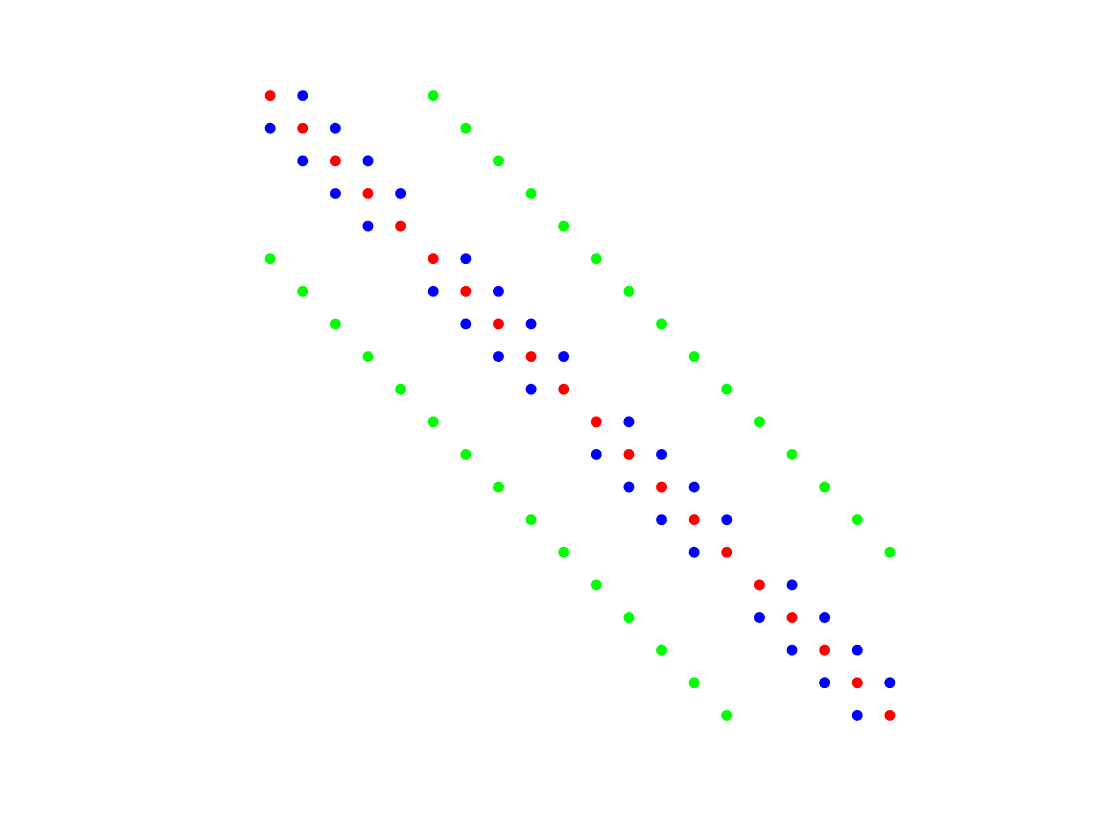
\includegraphics[width=0.5\textwidth]{discrete-laplacian}
    \caption{Second-order centered discrete Laplacian matrix}
    \label{fig:discrete-laplacian}
  \end{center}
\end{figure}
where the entries on the main diagonal (indicated in red) take the value $-\frac{2}{\Delta x^2}-\frac{2}{\Delta y^2}$, the entries on the subdiagonal and superdiagonal (indicated in blue) take the value $\frac{1}{\Delta x^2}$, and the entries on the outer diagonals (indicated in green) take the value $\frac{1}{\Delta y^2}$.

Note that the off-diagonals have missing entries corresponding to the boundary points. Traditional methods of implementing numerical PDE solvers require adjusting for the missing entries either by using ghost cells \todo{Cite} or by modifying the discretized source term $F$ \todo{Cite}. As the PDE and choice of discretization become more complicated, correctly incorporating boundary conditions becomes increasingly cumbersome and significantly hinders the ability to quickly explore the effectiveness of hand-crafted numerical schemes for solving PDEs.


\section{Problem Formulation}

The discretized version of Poisson's equation can now be expressed as
\begin{equation}
  A_* \vec{U} = \vec{F}
\end{equation}
where $A_*$ is the discrete Laplacian matrix shown in Figure \ref{fig:discrete-laplacian}.

\cite{dummy}

Smaller chance of bugs with declarative approach - provides reference implementation for comparison

Finite difference approximations (Crank-Nicolson, etc.), Laplacian boundary conditions, Poisson's equation, heat equation, analytical solutions

Note how problem is still convex


\section{Solutions}


\section{Simulations}


\section{Conclusion}


%%%%%%
%% To balance the columns at the last page of the paper use this
%% command:
%%
%\enlargethispage{-1.2cm}
%%
%% If the balancing should occur in the middle of the references, use
%% the following trigger:
%%
%\IEEEtriggeratref{3}
%%
%% which triggers a \newpage (i.e., new column) just before the given
%% reference number. Note that you need to adapt this if you modify
%% the paper.  The "triggered" command can be changed if desired:
%%
%\IEEEtriggercmd{\enlargethispage{-20cm}}
%%
%%%%%%

%%%%%%
%% References:
%% We recommend the usage of BibTeX:
%%
\bibliographystyle{IEEEtran}
\bibliography{bibliofile}
%%
%% BibTeX documentation can be obtained at:
%% http://www.ctan.org/tex-archive/biblio/bibtex/contrib/doc/
%%%%%%


\end{document}
